\subsection{Двухточечное скрещивание}\label{SetOfOperatorsAlgorithms:TwopointCrossover}

Идентификатор: \textbf{TwopointCrossover}.

Данный оператор скрещивания используется для бинарных векторов.

Пусть имеется два родителя (родительские хромосомы) $\overline{Parent}^1$ и $\overline{Parent}^2$. В двух случайных местах происходят разрывы между двумя позициями генов в обеих хромосомах. После этого хромосомы обмениваются частями, в результате чего образуются два потомка. Из них выбирается случайно один потомок, который и передается в качестве результата оператора скрещивания. То есть скрещивание происходит по формулам:

\begin{align}
\label{SetOfOperatorsAlgorithms:eq:TwopointCrossover}
&Crossover \left( \overline{Parent}^1, \overline{Parent}^2, DataOfCros\right)=Random \left(\left\lbrace \overline{Offspring}^1; \overline{Offspring}^2\right\rbrace  \right), \\
&r_1=Random\left( \left\lbrace 2; 3; \ldots; n\right\rbrace \right); \nonumber \\
&r_2=Random\left( \left\lbrace 2; 3; \ldots; n\right\rbrace \right); \nonumber \\
&R_1=\min \left( r_1, r_2\right) ; \nonumber \\
&R_2=\max \left( r_1, r_2\right) ; \nonumber \\
& \overline{Offspring}^1_i=\overline{Parent}^1_i, i=\overline{1,R_1-1};\nonumber\\
& \overline{Offspring}^1_i=\overline{Parent}^2_i, i=\overline{R_1,R_2-1};\nonumber\\
&  \overline{Offspring}^1_i=\overline{Parent}^1_i, i=\overline{R_2,n};\nonumber\\
& \overline{Offspring}^2_i=\overline{Parent}^2_i, i=\overline{1,R_1-1};\nonumber\\
& \overline{Offspring}^2_i=\overline{Parent}^1_i, i=\overline{R_1,R_2-1};\nonumber\\
&  \overline{Offspring}^2_i=\overline{Parent}^2_i, i=\overline{R_2,n};\nonumber\\
&\overline{Offspring}^1\in X, \overline{Offspring}^2\in X.\nonumber
\end{align}

\textbf{Пример.} Двухточечное скрещивание показано на рисунке:

\begin{figure} [H]
  \center
  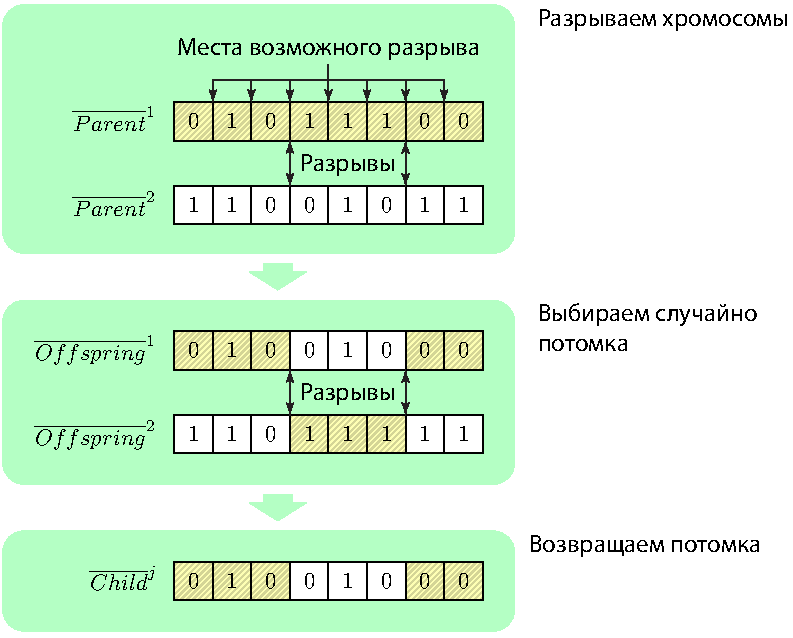
\includegraphics [scale=0.6] {TwopointCrossover}
  \caption{Механизм работы двухточечного скрещивания} 
  \label{SetOfOperatorsAlgorithms:img:TwopointCrossover} 
\end{figure}

$ DataOfCros $ не содержит каких-либо параметров относительно данного типа скрещивания.

В библиотеке \textbf{HarrixMathLibrary} данная селекция реализуется через функцию \textbf{THML\_TwopointCrossover}:

\href{https://github.com/Harrix/HarrixMathLibrary}{https://github.com/Harrix/HarrixMathLibrary}